\documentclass[10pt,dvipsnames]{beamer}
\usetheme[progressbar=frametitle,numbering=none]{metropolis}

% -------------------
% Tikz & PGF
% -------------------
\usepackage{tikz}
\usepackage{tikz-cd}
\usetikzlibrary{
	calc,
	decorations.pathmorphing,
	matrix,arrows,
	positioning,
	shapes.geometric
}

% -------------------
% Content
% -------------------

\title{Lösung zu: Artifacts}
\author{Bernhard Germann, Massoud Vincent Shahriyari}
\subtitle{Lösungsskizze zu Aufgabe 6d}
\begin{document}
  \begin{frame}
    \frametitle{AlgMetP SS 2020}
    \titlepage
  \end{frame}

  \begin{frame}
    \frametitle{Aufgabenstellung}
    \begin{itemize}
      \item \textbf{Gegeben:}
      \begin{itemize}
        \item $n_w$ Krieger
        \item $n_s$ Zauber
        \item $n_m$ Magier
        \item $n_a$ Artefakte
        \item Magier verbrauchen Artefakte, um Zauber zu wirken
        \item Ein Krieger ist nur mit manchen Zaubern kompatibel
        \item Auf den Krieger $w_i$ können höchstens $b_i$ Zauber gewirkt werden
        \item Ein Magier ist nur mit manchen Zaubern kompatibel
        \item Ein Magier ist nur mit manchen Artefakten kompatibel
        \item Ein Artefakt ist entweder episch oder normal
        \item Von Artefakt $a_i$ gibt es $e_i$ Exemplare
        \item Ein Magier verbraucht 3 identische normale Artefakte oder 1 episches Artefakt, um einen Zauber zu wirken
      \end{itemize}
      
      \item \textbf{Frage:} Was ist die maximale Anahl an Zaubern, die unter den gegebenen Constraints gewirkt werden können?
      
      \item \textbf{Ansatz:} Modelliere das Problem als Flussgraphen und wende dann den Max-Flow Algorithmus an.
    \end{itemize}
  \end{frame}
  
  \begin{frame}
  \frametitle{Lösungsskizze}
  \begin{itemize}
    \item Flussgraph $G=(V,E)$ und Gewichtsfunktion $f$ definiert definiert durch:
      \begin{itemize}
        \item Quelle $s\in V$, Ziel $t \in V$
        \item Krieger $a_1,\dots,a_{n_a}\in V$
        \item Krieger $m_1,\dots,m_{n_m}\in V$
        \item Krieger $s_1,\dots,s_{n_s}\in V$
        \item Krieger $w_1,\dots,w_{n_w}\in V$
        \item $(s,a_i)\in E$
        \item Wenn $a_i$ normal, dann $f(s,a_i)=\lfloor\frac{e_i}{3}\rfloor$
        \item Wenn $a_i$ episch, dann $f(s,a_i)=e_i$
        \item $(a_i,m_j)\in E$, falls $a_i,m_j$ kompatibel, $f(a_i,m_j)=\infty$
        \item $(m_i,s_j)\in E$, falls $m_i,s_j$ kompatibel, $f(m_i,s_j)=\infty$
        \item $(s_i,w_j)\in E$, falls $s_i,w_j$ kompatibel, $f(s_i,w_j)=\infty$
        \item $(w_i,t)\in E$
        \item $f(w_i,t)=b_i$
      \end{itemize}
    \item Die Lösung ist $Max\mbox{-} Flow(G,s,t)$
  \end{itemize}
    
  \end{frame}
  
  \begin{frame}
    \frametitle{Flussgraph zum Beispiel-Input 1, Testcase 2}
    \begin{center}
      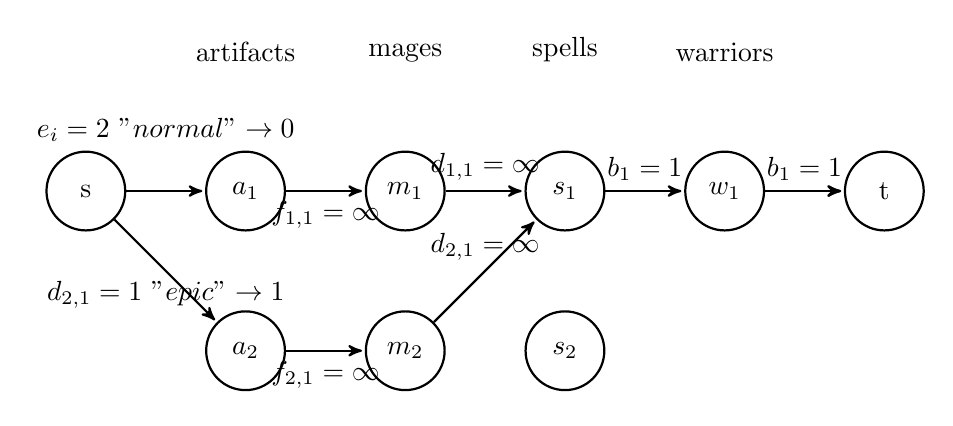
\begin{tikzpicture}[->,>=stealth',shorten >=1pt,node distance=70pt,
        thick,main
       node/.style={circle,draw,minimum size=1cm}]
        \node[main node] (s) {s};
        \node[main node] (a11) [right = 1cm of s] {$a_1$};
        \node[main node] (a12) [below = 1cm of a11] {$a_2$};
        \node [above =1cm of a11] (a) {artifacts};
        \node[main node] (m11) [right = 1cm of a11] {$m_1$};
        \node[main node] (m12) [below = 1cm of m11] {$m_2$};
        \node [above = 1cm of m11] {mages};
        \node[main node] (s11) [right = 1cm of m11] {$s_1$};
        \node[main node] (s12) [below = 1cm of s11] {$s_2$};
        \node [above = 1cm of s11] {spells};
        \node[main node] (w11) [right = 1cm of s11] {$w_1$};
        \node [above = 1cm of w11] {warriors};
        \node[main node] (t) [right =1cm of w11] {t};
        
          \draw (s) edge node[above = 0.5cm]{$e_{i} = 2\ "normal" \rightarrow 0$} (a11);
          \draw (s) edge node[below = 0cm]{$d_{2,1} = 1\ "epic" \rightarrow 1$} (a12);
          
          \draw (a11) edge node[below]{$f_{1,1} = \infty$} (m11);
          \draw (a12) edge node[below]{$f_{2,1} = \infty$} (m12);

          \draw (m11) edge node[above]{$d_{1,1} = \infty$} (s11);
          \draw (m12) edge node[above]{$d_{2,1} = \infty$} (s11);

          \draw (s11) edge node[above]{$b_1 = 1$} (w11);
          
          \draw (w11) edge  node[above]{$b_1 = 1$} (t);
          \draw (w11) edge (t);
          
      \end{tikzpicture}
    \end{center}
  \end{frame}
  
  \begin{frame}
    \frametitle{Zusammenfassung}
    \begin{itemize}
      \item \textbf{Art des Problems:}
      \begin{itemize}
        \item Optimierungsproblem
        \item Graphenproblem
      \end{itemize}
    \end{itemize}
    
    \begin{itemize}
      \item \textbf{Algorithmische Methoden zur Lösung:}
      \begin{itemize}
        \item Max-Flow-Algorithmus (z.B. Edmonds-Karp Algorithmus)
      \end{itemize}
    \end{itemize}
  \end{frame}
\end{document}
